%! Author = Frederik Bußmann
%! Date = 22.06.2023

\section{Fachlicher Hintergrund} \label{sec:02-background}

Für die Erarbeitung einer geeigneten \acrshort{ci}-Strategie wird zunächst ein Einblick in die Disziplin des
Continuous-Software-Engineering gegeben.
Anschließend werden die Begrifflichkeiten und Prinzipien von Continuous Integration definiert und weitere
relevante Technologien und Bereiche für die Nutzung von\ \acrshort{ci} erläutert.
Darüber hinaus wird eine Übersicht über die Funktionen und Mechanismen der Shopware-Plattform gegeben.

\subsection{Continuous Software Engineering} \label{subsec:02-background-1}

Continuous-Software-Engineering fasst die Prinzipien der Continuous Integration (\acrshort{ci}),
Continuous Delivery (\acrshort{cde}), und Continuous Deployment (\acrshort{cd}) zusammen.
Shahin et al.\ definieren den Begriff als einen Bereich der Softwareentwicklung, bei dem es um die Entwicklung,
Auslieferung und das schnelle Feedback von Software und Kunde geht.
Die Disziplin umfasst Geschäftsstrategie und Planung, sowie Entwicklung und den Betrieb der Software.
\footpartcite[3910--3911]{tools-and-practises}
Diese kontinuierliche Integrierung von Software ist sehr kompatibel mit den häufigen iterationen in der agilen
Softwareentwicklung und wurde unter anderem durch die agile Methodik des Extreme Programming bekannt.
\footpartcite{fitzgerald}
Nachfolgend werden die Bereiche der agilen Softwareentwicklung und der \acrshort{ci},\ \acrshort{cde} und \acrshort{cd}
kurz erläutert.

\subsubsection{Agile Software Development}

Agile Softwareentwicklung ist ein Ansatz zur Softwareentwicklung, der auf Flexibilität und Kundeninteraktion setzt.
Im Gegensatz zu traditionellen, plangetriebenen Methoden, die die Anforderungen und Lösungen am Anfang des Projekts
festlegen, erlaubt die agile Methodik Änderungen und Anpassungen während des gesamten Entwicklungsprozesses.
Dies wird durch iterative Entwicklung und regelmäßiges Feedback erreicht.
Zu den wichtigsten Prinzipien der agilen Softwareentwicklung gehören die kontinuierliche Auslieferung von Software,
Offenheit für sich ändernde Anforderungen und enge Zusammenarbeit zwischen Teams und Entwicklern.
\footpartcite{agile-manifesto}
Gren und Lenberg fassen Agile als die Reaktionsfähigkeit im Hinblick auf sich ständig ändernde Anforderungen
und Umgebungen zusammen.\footpartcite{agile}

\subsubsection{Continuous Integration}

Continuous Integration (\acrshort{ci}) ist ein Softwareentwicklungsprozess, bei dem Entwickler ihre Änderungen
regelmäßig, oft mehrmals täglich, in ein gemeinsames Repository integrieren.
Jede dieser Integrationen wird dann von einem automatisierten Build-System überprüft, um sicherzustellen, dass die
Änderungen mit der bestehenden Codebase kompatibel sind und keine Fehler verursachen.
Dieser Prozess ermöglicht es Teams, Probleme frühzeitig zu erkennen und zu beheben, was die Qualität der Software
verbessert und die Zeit bis zur Auslieferung der Software reduziert.\footpartcite{fowler}

\subsubsection{Continuous Delivery}

Continuous Delivery (\acrshort{cde}) erweitert das Konzept der Continuous Integration, indem es sicherstellt, dass die
Software stetig in einem Zustand ist, der sicher in die Produktionsumgebung ausgerollt werden kann.
Dies wird durch das Einführen von Integrationstests, die die Funktionalität der vollständigen Software inklusive aller
Module testen, erreicht.
Das Ziel von\ \acrshort{cde} ist es, den Prozess der Softwareauslieferung zu beschleunigen und zuverlässiger zu machen,
indem menschliche Fehler minimiert und schnelles Feedback über Probleme in der Produktionsumgebung ermöglicht wird.
\footpartcite{humble}

\subsubsection{Continuous Deployment}

Continuous Deployment (\acrshort{cd}) ist der nächste Schritt nach Continuous Delivery.
Bei\ \acrshort{cd} wird jede Änderung, die den automatisierten Testprozess besteht, automatisch in die
Produktionsumgebung eingespielt.\footpartcite[3911]{tools-and-practises}
Dies bedeutet, dass neue Features und Updates mehrmals täglich an die Endbenutzer ausgeliefert werden können, was eine
schnelle Reaktion auf Marktbedingungen und Kundenfeedback ermöglicht.
Es ist jedoch zu beachten, dass\ \acrshort{cd} eine hohe Reife der Entwicklungsprozesse und Testautomatisierung
erfordert, um die Anzahl der in der Produktionsumgebung aufkommenden Fehler zu minimieren.
Der Zusammenhang zwischen Continuous Integration, Delivery und Deployment wird in Abbildung\ \ref{fig:ci-cde-cd}
aufgezeigt.

\begin{figure}[H]
    \centering
    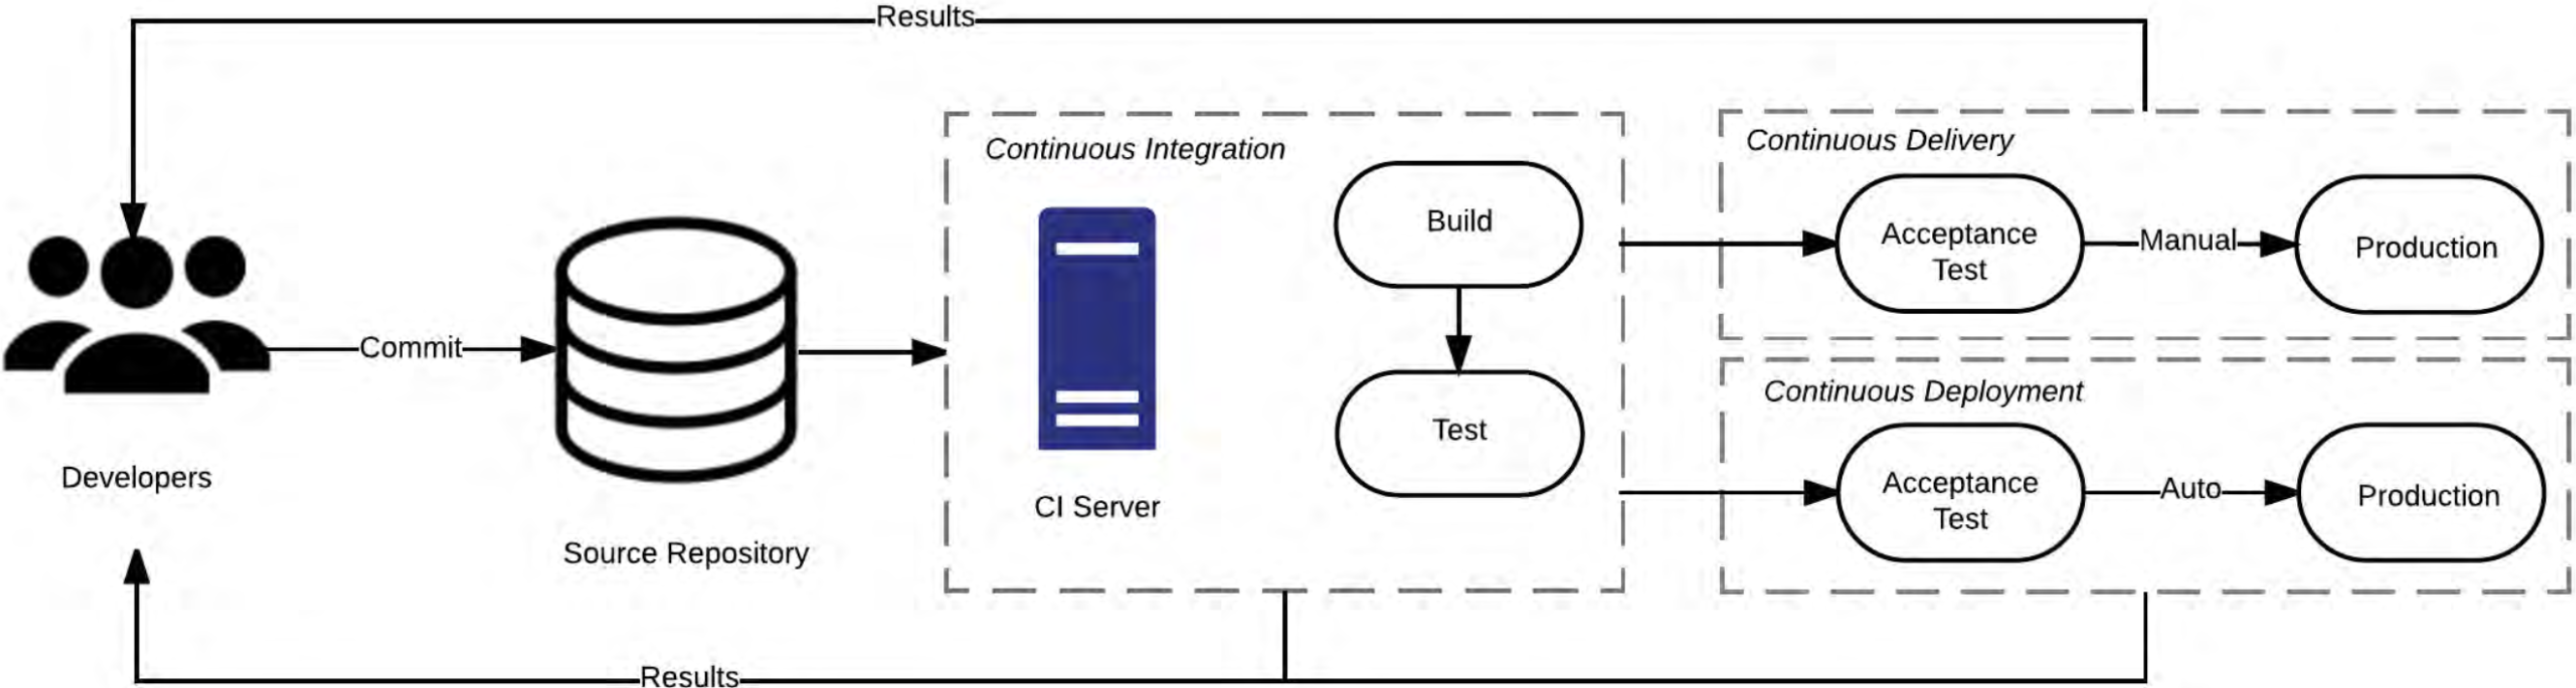
\includegraphics[width=0.91\textwidth]{images/content/ci-cde-cd}
    \captioncite[Übernommen von]{tools-and-practises}{Zusammenhang zwischen \acrshort{ci}, \acrshort{cde} und \acrshort{cd}}
    \label{fig:ci-cde-cd}
\end{figure}

\subsection{Begrifflichkeiten und Prinzipien von Continuous Integration} \label{subsec:02-background-2}

% @TODO: Irgendwo noch DevOps erklären (?)

Um die Bedeutung und den Nutzen von Continuous Integration und des Continuous-Software-Engineering für die
Softwareentwicklung nachvollziehen zu können, ist es hilfreich, einen Blick auf die historische Entwicklung und die
grundlegenden Prinzipien der\ \acrshort{ci} zu werfen.
Ein Kernprinzip hinter Continuous Integration wurde bereits im Jahr 1991 von Grady Booch definiert.
Hierbei werden Software-Releases nicht als ein großes Ereignis betrachtet, sondern regelmäßig durchgeführt, wobei
die vollständige Software stetig größer wird.\footpartcite{booch}
Kent Beck popularisierte im Jahr 1998 die Disziplin des\ \glqq Extreme Programming\grqq, wobei großer Wert auf das frühe
und regelmäßige Testen und Integrieren der entwickelten Komponenten einer Software gelegt wird.
Beck behauptet hierbei, dass ein Feature, für welches es keine automatisierten Tests gibt, auch nicht funktioniert.
\footpartcite[2--4]{extreme-programming}
Im Jahr 2006 fasste Software-Entwickler Martin Fowler einige Bereiche dieser Methodiken in dem Artikel
\glqq Continuous Integration\grqq\ unter dem gleichnamigen Begriff zusammen.
Fowler beschreibt\ \acrshort{ci} als einen Prozess, bei dem Teammitglieder ihre Arbeit regelmäßig Integrieren,
wobei Integration als der Build-Prozess, inklusive automatisierter Tests, für die vollständige Software mitsamt der
erarbeiteten Änderungen zu verstehen ist.\footpartcite{fowler}
Ein grundlegendes Ziel dieser Vorgehensweise ist, neben der frühzeitigen Erkennung von Fehlern im Quellcode durch
automatisierte Tests und\ \acrshort{qa}-Prüfungen, die Reduzierung der\ \glqq Cycle Time\grqq, welche die Zeitspanne von
der Entwicklung eines Features bis zum Erhalten des Kundenfeedbacks nach dessen Auslieferung beschreibt.
\footpartcite[2580]{benefits-challenges}
In 2010 betonen Humble und Farley die Wichtigkeit von\ \acrshort{ci} und behaupten, dass Software ohne Continuous
Integration als defekt gilt, bis sie als funktionierend nachgewiesen wird, während mit\ \acrshort{ci} Software mit
jeder erfolgreich integrierten Änderung als funktionierend bewiesen wird.\footpartcite[56]{humble}
Über Zeit hat sich\ \acrshort{ci} als essenzielle Praktik in der Software-Welt etabliert.
Im Jahr 2016 zeigte eine Analyse von $34.544$ auf der Plattform GitHub verwalteten Open-Source-Projekten, dass 40\% der
Projekte\ \acrshort{ci} einsetzen.
Bei den populärsten 500 analysierten Projekten lag der Anteil bei 70\%.\footpartcite[428--429]{ci-usage}
Da die erfolgreiche Implementierung von Continuous Integration auf der Kombination von verschiedenen Methoden zur
Verwaltung von Softwareprojekten fußt, werden im Folgenden einige dieser Schlüsselaspekte aufgezeigt:

\begin{itemize}
    \item {
        \textbf{Regelmäßige Integration}\par
        Die namensgebende Methodik der\ \acrshort{ci} ist das regelmäßige Integrieren von Software und damit Verbunden
        ist der Software-Release.
        In der traditionellen Softwareentwicklung wird der Release als ein einmaliges, großes Ereignis betrachtet.
        Als Integration wird der Prozess des Einbindens einer einzeln entwickelten Komponente in die bisher bestehende
        Gesamtheit einer Software bezeichnet, wobei der Release das Zusammenfinden aller Komponenten und das Ausführen
        des Build-Prozesses bis hin zur fertigen, ausführbaren und auslieferbaren Software beschreibt.
        In der Vergangenheit wurde bei einem Release jede Einzelkomponente der Software manuell integriert und getestet,
        wobei dies als eigene Phase in der Entwicklung einer Applikation galt.
        In einem \acrshort{ci}-gestützten Projekt wird der Prozess des Software-Releases vollständig automatisiert,
        sodass jedes Teammitglied eine entwickelte Komponente schnell Integrieren und einen Software-Build erzeugen
        kann, was sich positiv auf die Cycle Time auswirkt.
        In einem Build-Prozess erzeugte Dateien, welche die fertig gebaute Software ausmachen, werden dabei als\ \glqq
        Artifact\grqq\ betitelt.\footpartcite[2580]{benefits-challenges}
        Fowler empfiehlt hierbei, dass ein entwickeltes Feature erst nach der vollständigen Integration durch einen
        erfolgreichen Build als fertig angesehen werden soll.\footpartcite{fowler}
        In der Regel finden das Bauen und Testen der Software in einer\ \glqq Pipeline\grqq\ statt, welche die genutzten
        \acrshort{ci}-Tools wie Test-Suites und Static-Code-Analysis ausführt.\footpartcite[2571]{benefits-challenges}
    }

    \item {
        \textbf{Automatisierte Tests}\par
        Neben der regelmäßigen Integrierung von Code gelten automatisierte Software-Tests und Quality-Checks als ein
        wichtiger Aspekt von\ \acrshort{ci}.
        Hierbei werden oftmals Unit-Tests verwendet, welche eine einzelne Softwarekomponente auf
        ihre Funktion prüfen, abgekapselt von anderen Komponenten.\footpartcite[280]{test-driven-development}
        Wenn ein Test fehlschlägt, wird in der Regel die Pipeline unterbroche.
        Neben den typischerweise schnell durchlaufenden Unit-Tests, die aufgrund ihrer isolierten Natur spezifische
        Komponenten prüfen, können nach dem Build-Prozess umfassende End-To-End-Tests für die gesamte Software
        durchgeführt werden.
        Diese Systemübergreifenden Tests, welche das Zusammenspiel verschiedener Komponenten testen, erhöhen zwar die
        Dauer des Test-Prozesses, können aber wichtige Einsicht in die Qualität der Software gewähren.
        \footpartcite{fowler}
        Automatisierten Tests in einer\ \acrshort{ci}-Pipeline können insgesamt dabei helfen, Fehler in eingeführtem
        Quellcode zu finden.\footpartcite[2572]{benefits-and-challenges}
        Oftmals kommen auch Static-Code-Analysis Tools zum Einsatz, um eine Pipeline bei Unstimmigkeiten in der Syntax
        des eingeführten Codes abzubrechen.
        Diese Programme können zusätzliche Qualitätsprüfungen und Coding-Standards in ein Projekt einführen.
        \footpartcite[338]{static-analysis}
    }

    \item {
        \textbf{Reproduzierbarkeit}\par
        Ein weiterer zentraler Aspekt von Continuous Integration ist die Reproduzierbarkeit der \acrshort{ci}-Pipeline.
        In einem \acrshort{ci}-Umfeld werden der Build- und Testing-Prozess vollständig automatisiert und
        standardisiert, was bedeutet, dass diese unter den gleichen Bedingungen und mit den gleichen Ergebnissen
        wiederholt werden können.
        Dies ist von entscheidender Bedeutung, um sicherzustellen, dass die Software in verschiedenen Umgebungen
        (z.B.\ Entwicklung, Test, Produktion) konsistent funktioniert.
        Durch das Zentralisieren der Software und der \acrshort{ci}-Tools in einer Versionierungs-Software, in
        Verbindung mit dem Automatisieren des Build- und Testing-Prozesses, wird das Wiederherstellen von früheren
        Ständen in der Entwicklung und das Nachvollziehen von Fehlern im Entwicklungsprozess vereinfacht.
        \footpartcite[74--75]{duvall}
    }

    \item {
        \textbf{Transparenz}\par
        Transparenz in einem\ \acrshort{ci}-Prozess bedeutet, dass alle Aspekte des Entwicklungsprozesses sichtbar und
        verständlich sind, sowohl innerhalb des Entwicklungsteams als auch für andere Stakeholder.
        Sie ermöglicht eine klare Sicht auf den aktuellen Stand des Projekts, einschließlich der Qualität des Codes,
        der Fortschritte und möglicher Probleme.
        Durch den Einsatz von\ \acrshort{ci} und der Automatisierung des Build- und Test-Prozesses können Teammitglieder
        schnell Feedback über den Status von Änderungen an der Codebase erhalten.
        Wenn ein Problem auftritt, z.B.\ ein Test fehlschlägt oder ein Build abbricht, wird das Team sofort
        benachrichtigt, sodass das Problem schnell behoben werden kann.
        Dies reduziert die Zeit und den Aufwand, die benötigt werden, um Fehler zu finden und zu beheben, und verbessert
        die Qualität der Software.
        Darüber hinaus fördert das schnelle Feedback die Kommunikation und Zusammenarbeit im Team, da alle Mitglieder
        ständig über den Status des Projekts informiert sind.
        \footpartcite[2573]{benefits-challenges}\textsuperscript{,}\footpartcite[26--27]{adept}
    }
\end{itemize}

Die vorgestellten\ \acrshort{ci}-Praktiken bauen auf unterschiedlichen Technologien und Konzepten auf, die für das
Betreiben von Continuous Integration eine Rolle spielen.
Um die Praktiken der Continuous Integration vollständig zu verstehen und effektiv umzusetzen, ist es
unerlässlich, die zugrunde liegenden Technologien und Konzepte zu betrachten, die die Basis für die Implementierung von
\acrshort{ci} in einem Softwareprojekt bilden.
Dazu gehören Themen wie Version-Control-Systems, Pipelines, Containerization, Software-Testing und
Static-Code-Analysis.
Im Folgenden werden einige dieser Themen untersucht, um ein umfassendes Verständnis der Mechanismen und Werkzeuge zu
vermitteln, die für die erfolgreiche Anwendung von Continuous Integration erforderlich sind.

\subsubsection{Version-Control-Systems}

% @TODO: Branching-Strategien erklären

Das Verwalten verschiedener Versionsstände von Software wird durch sogenannte Version-Control-Systems (\acrshort{vcs})
ermöglicht.
Es gibt verschiedene Implementierungen von\ \acrshort{vcs}, namentlich unter anderem Git, Mercurial, Subversion und
weitere.
Ein\ \acrshort{vcs} speichert den gesamten Quellcode eines Projekts in einem eigenen\ \glqq Repository\grqq.
\footpartcite[381--385]{duvall}
Innerhalb desselben Repositories können verschiedene Versions-Historien in sogenannten\ \glqq Branches\grqq\ gespeichert
werden.
Der aktuelle Stand eines Branches kann dabei kopiert werden und daran vorgenommene Revisionen können anschließend wieder
in einen Branch des Repositories integriert werden.
Versionskontroll-Software ermöglicht es außerdem, verschiedene Versionen in Form von Branches zusammenzuführen.
Der Prozess des Zusammenführens verschiedener Branches wird hierbei als\ \glqq Merge\grqq\ bezeichnet.
Die Nutzung eines\ \acrshort{vcs} in welchem verschiedene Branches angelegt werden können, ermöglicht Teammitgliedern
die gleichzeitige Arbeit an einer einzelnen Codebase ohne sich dabei gegenseitig zu beeinflussen.
\footpartcite[388--390]{duvall}
Fowler setzt für die Nutzung von\ \acrshort{ci} das Führen eines Source-Repositories voraus, welches die
Projekt-Software, inklusive aller dazugehörigen Build- und Testing-Konfigurationen, verwaltet.\footpartcite{fowler}

\subsubsection{Pipelines}

Um die in einer Versionskontroll-Software eingeführten Code-Änderungen automatisiert bauen, testen und ausliefern zu
können, wird eine ausführende Umgebung für diese Prozesse benötigt.
In einem\ \acrshort{ci}-Prozess werden hierfür Pipelines eingesetzt, welche zum Ausführen von Befehlen und Prozessen
zur automatischen Integration und dem Testen von Code genutzt werden.
\footpartcite[2571]{benefits-challenges}
Sie werden durch sogenannte Pipeline- oder Task-Runner verwaltet und können verschiedene Aufgaben verrichten,
welche durch das Ausführen von Befehlen innerhalb sogenannter\ \glqq Jobs\grqq\ durchgeführt werden.
Pipelines können mehrere Jobs starten, teilweise auch parallel, wobei nacheinander laufende Jobs voneinander
Abhängig sein und Artifacts für nachfolgende Jobs zwischengespeichert werden können.
Pipelines spielen durch das kontinuierliche Integrieren von entwickeltem Code eine integrale Rolle bei der Reduzierung
der Cycle Time\footpartcite{fowler} und sind somit wichtig zum Erreichen des Ziels $Z_1$ der Arbeit.
Eine Pipeline in einem\ \acrshort{ci}-Prozess wird in der Regel bei jeder Änderung am Quellcode des Source-Repositories
gestartet.\footpartcite[3--4]{duvall}
Die Durchlaufzeit einer\ \acrshort{ci}-Pipeline sollte dabei möglichst gering bleiben, da viele Entwickler
auf das erfolgreiche Durchlaufen der Pipeline warten, bevor sie mit der nächsten Aufgabe beginnen.
Eine grobe Richtlinie für die maximale Dauer einer Pipeline ist die Zehn-Minuten-Marke.
\footpartcite[87--88]{duvall}

\subsubsection{Containerization}

Um die zum Bauen, Testen und Ausliefern von Software in einem\ \acrshort{ci}-Projekt benötigten Pipelines nutzen zu
können, wird eine isolierte und reproduzierbare ausführende Umgebung benötigt.
In der Vergangenheit wurden für solche isolierten Umgebungen hauptsächlich\ \glqq Virtual
Machines\grqq\ (\acrshort{vm}s) verwendet.
\acrshort{vm}s nutzen hierbei einen sogenannten\ \glqq Hypervisor\grqq, welcher die Hardware eines physischen Computers
emulieren kann, sodass mehrere Betriebssysteminstanzen und die darin verwalteten Applikationen gleichzeitig auf einem
einzigen System ausführbar sind.\footpartcite[54--55]{docker}
Containerization ist eine modernere Technologie, die einen Performance-Zuwachs gegenüber \acrshort{vm}s bieten kann.
\footpartcite{docker-performance}
Die hierbei genutzten\ \glqq Container\grqq\ sind eigenständige, ausführbare Pakete, die alles enthalten, was für den
Betrieb einer Anwendung erforderlich ist, einschließlich Code, Laufzeitumgebung, Bibliotheken und Systemtools.

\begin{figure}[H]
    \centering
    \begin{minipage}{0.4\textwidth}
        \centering
        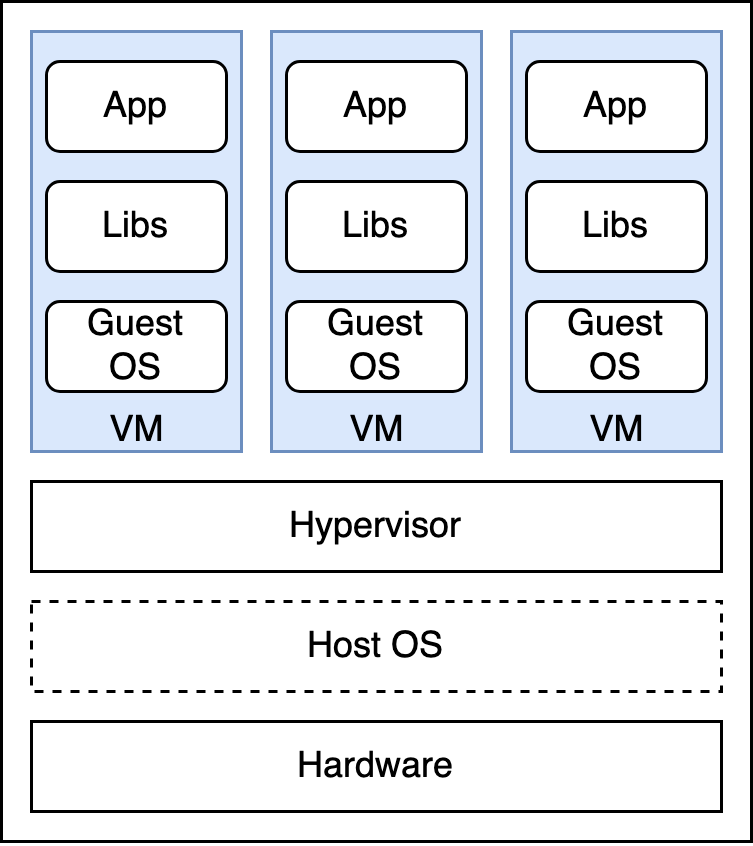
\includegraphics[width=\linewidth]{images/content/vm-architecture}
        \captionsetup{justification=raggedright,singlelinecheck=false}%
        \vspace{-0.7cm}%
        \caption*{(a)}
    \end{minipage}%
    \hspace{0.075\textwidth}%
    \begin{minipage}{0.4\textwidth}
        \centering
        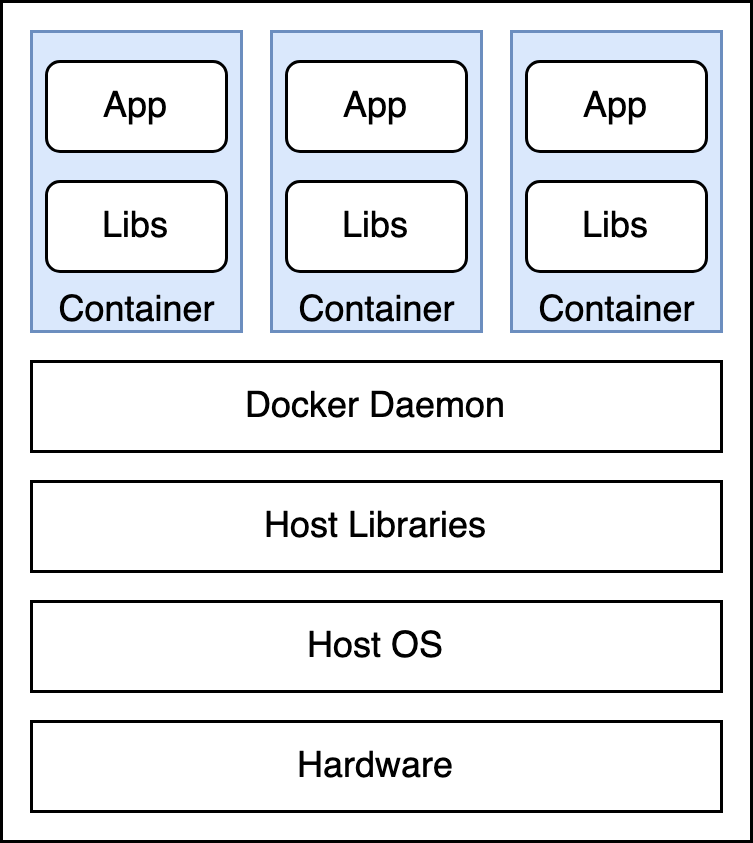
\includegraphics[width=\linewidth]{images/content/container-architecture}
        \captionsetup{justification=raggedright,singlelinecheck=false}%
        \vspace{-0.7cm}%
        \caption*{(b)}
    \end{minipage}
    \captioncite[Eigene Darstellung nach]{docker}{Visualisierung der Hypervisor- und Container-Architektur}
    \label{fig:vm-container-architecture}
\end{figure}

Während \acrshort{vm}s zur Ausführung einen Hypervisor und vollständige Betriebssysteminstanzen benötigen, teilen sich
Container die Ressourcen eines einzelnen Betriebssystems und isolieren so die Anwendung von der zugrunde liegenden
Infrastruktur.
Ein Container ist hierbei die laufende Instanz eines Container-Images, welches den Aufbau des Containers inklusive
Abhängigkeiten und installierter Software speichert.
Containerization erleichtert also das Vereinheitlichen verschiedener Umgebungen in \acrshort{ci}-Projekten, indem es
Abhängigkeiten und Konfigurationen in einem Container kapselt.\footpartcite[2576]{benefits-challenges}
Dies bietet Entwicklern und Testern eine erhöhte Effizienz und Flexibilität, da sie sich darauf verlassen können, dass
die Software in jeder Umgebung identisch funktioniert.
In Abbildung\ \ref{fig:vm-container-architecture} werden die Architekturen von Hypervisor und Container
gegenübergestellt.
Die Visualisierung zeigt im linken Teil den Aufbau eines Systems, in dem ein Hypervisor zum emulieren von
Hardware-Ressourcen verwendet wird (a).
Die Technologie kann hierbei auf einem bereits installierten Host-Betriebssystem (Host\ \acrshort{os}) oder ganz ohne
\acrshort{os} betrieben werden.
Einzelne\ \acrshort{vm}s die durch den Hypervisor betrieben werden können, nutzen hierbei jeweils ein eigenes
Gast-Betriebssystem (Guest\ \acrshort{os}).
Im Kontrast dazu steht die Container-Architektur, welche das Betreiben eines Host\ \acrshort{os} voraussetzt und
dessen Ressourcen zur Ausführung isolierter Container-Instanzen verwendet (b).
Das Ausführen der Container wird dabei durch eine Container-Engine übernommen, im Falle der Docker-Technologie wird
dies durch einen eigenen Hintergrundprozess (Docker Daemon) ermöglicht.

\subsubsection{Software-Testing}

Wenn eine ausführende Umgebung für das Bauen und Testen von Software besteht, können Software-Tests in den
\acrshort{ci}-Prozess eingeführt werden.
Durch manuelle und automatisierte Tests kann ein Software-Produkt auf verschiedene Funktionsbereiche überprüft werden.
Da manuelle Tests einen hohen Zeitaufwand darstellen können, wird Testautomatisierung in der agilen Softwareentwicklung
als wichtige Aktivität angesehen.
Besonders bei repetitiven Aufgaben zum Reproduzieren vordefinierter Systemfunktionalitäten wirken automatisierte
Tests effizienzsteigernd.\footpartcite[440]{agile-testing}
Sie müssen hierbei nur einmal angelegt werden und können anschließend beliebig oft und ohne weitere Aufwände erneut
ausgeführt werden.
In\ \acrshort{ci}-Projekten werden automatisierte Tests oftmals eingesetzt, um Probleme bei der
Einführung von Features mit vorher entwickelter Logik zu vermeiden und um Fehler im Entwicklungsprozess früher
entdecken zu können.
Häufiges, automatisiertes Testing in der\ \acrshort{ci} kann sich positiv auf die Qualität der entwickelten Software
auswirken.\footpartcite[281]{test-driven-development}\textsuperscript{,\ }\footpartcite[2570]{benefits-challenges}
\\
Nachfolgend werden verschiedene Arten von Tests in der Softwareentwicklung vorgestellt:
\footpartcite[23--24]{software-testing}

\begin{itemize}
    \item {
        \textbf{Unit-Tests}\par
        Unit-Tests prüfen das verhalten von einzelnen Programm-Einheiten.
        Eine Programm-Einheit oder Prozedur stellt eine oder mehrere zusammenhängende Anweisungen in Form von Code dar,
        welche durch andere Teile der Software namentlich aufgerufen werden können.
        Durch Unit-Tests werden also die Implementierungsschritte eines Software-Programms einzeln geprüft.
    }

    \item {
        \textbf{Module-Tests}\par
        Ein Modul besteht aus einer Sammlung zusammengehöriger Programm-Einheiten die in einer Datei, einem Paket oder
        einer Klasse zusammengefasst sind.
        Module-Tests, auch Component-Tests genannt, zielen darauf ab, diese Module isoliert zu bewerten, im Hinblick auf
        die Interaktionen zwischen den Einheiten und ihren dazugehörigen Datenstrukturen.
        In der Praxis können Unit- und Module-Tests zusammengefasst als Prüfung der eigentlichen Implementierung eines
        Programms betrachtet werden.\footpartcite[441]{agile-testing}
    }

    \item {
        \textbf{Integration-Tests}\par
        Integration-Tests fokussieren sich auf die Integration verschiedener Module einer Software.
        Sie prüfen das Zusammenspiel von unterschiedlichen Komponenten des Programms und stellen so sicher, dass die
        Kommunikation zwischen verschiedenen Bereichen der Applikation korrekt verläuft.
        Integrations-Tests stützen sich dabei auf die Annahme, dass die Module selbst bereits vollständig funktionieren.
    }

    \item {
        \textbf{System-Tests}\par
        Ähnlich wie Integration-Tests, prüfen System-Tests mehrere Komponenten eines einzelnen Systems auf ihre
        Zusammenarbeit.
        System-Tests grenzen sich hierbei allerdings durch ihren Bezug auf vorher definierte Produktanforderungen ab.
        Sie prüfen ob ein Programm in gänze funktioniert, wobei der Erfolg der Tests aus der Erfüllung von
        vordefinierten, geschäftsseitigen Anforderungen an das Programm besteht.
        Diese Art von Test wird auch als\ \glqq Functional Test\grqq\ bezeichnet.\footpartcite[441]{agile-testing}
    }

    \item {
        \textbf{Acceptance-Tests}\par
        Acceptance-Tests werden manuell ausgeführt.
        Sie prüfen, ob die Bedürfnisse des Projekt-Kunden durch die fertiggestellte Software abgedeckt werden.
        Hierbei werden also Tests aus der Sicht der Kunden oder vom Kunden selbst durchgeführt, welche fehlschlagen
        wenn dessen Anforderungen an das Programm nicht erfüllt werden.
    }
\end{itemize}

Durch diese verschiedenen Test-Arten kann ein großer Bereich der zu testenden Software und dessen Codebase abgedeckt
werden.
Da bereits erstellte Tests immer wieder verwendet werden können, werden diese oftmals eingesetzt um zu prüfen, ob neu
eingeführter Code diese bestehenden Tests fehlschlagen lässt.
Dieser Einsatz von existierenden Tests zur Sicherstellung der Funktionalität des Systems wird Regression-Testing
genannt und stellt einen wichtigen Aspekt des automatisierten Prüfens von Software in einem\ \acrshort{ci}-Kontext dar.
\footpartcite[53--54]{duvall}
Um beim Ausführen von Tests etwaige Abhängigkeiten die zur Ausführung des Codes innerhalb Test benötigt werden zu
umgehen, werden\ \glqq Mocks\grqq\ eingesetzt.
Ein Mock stellt eine Nachahmung der Vorgehensweise einer Abhängigkeit dar, so kann zum Beispiel das Verhalten
einer Datenbank oder eines anderen System-Moduls simuliert werden, ohne diese als Service im Testing-Prozess zu
benötigen.\footpartcite[299--300]{software-testing}
Zur Bewertung der Effektivität und Qualität von erstellten Software-Tests gibt es verschiedene Ansätze, ein
wichtiger Indikator ist jedoch die Test-Abdeckung.
Der Anteil von durch Tests abgedeckten Klassen und Funktionen im Kontrast zu der Anzahl an
ungetesteten Komponenten der Software wird als Abdeckung oder\ \glqq Coverage\grqq\ bezeichnet.
\footpartcite[132--133]{duvall}
Neben Test-Coverage können noch weitere Metriken, wie Mutation-Tests zur Bestimmung der Qualität von Tests genutzt
werden.
Hierbei wird der zu testende Source-Code verändert, oder mutiert, und dieser abgeänderte Code mit einem
bestehenden Test-Set geprüft.
Wenn die mutierte Variante des Codes durch das Test-Set aufgedeckt wurde, indem der Test fehlschlägt, wird
der mutierte Code, auch Mutant genannt, als eliminiert betrachtet.
Durch Mutation-Testing können Schwachstellen in Software-Tests gefunden werden und die Qualität der bestehenden
Tests eines Projekts gemessen werden.\footpartcite[242]{software-testing}

\subsubsection{Static-Code-Analysis}

Neben automatisiertem Testing ist das statische Analysieren des Codes ein weiterer wichtiger Aspekt für die
Qualitätskontrolle von Software in einer \acrshort{ci}-Umgebung.
Wo Tests nur die Ergebnisse des Ausführens von Komponenten und Funktionen messen, können statische
Code-Analysis-Tools die Struktur des Codes und die Einhaltung von vorgegebenen Standards bewerten.
Eine laufende \acrshort{ci}-Pipeline kann so bei der Einführung von Code, welcher nicht dem vorgegebenen Coding-Standard
entspricht, abgebrochen werden.
Dies zwingt die Entwickler eines Projekts dazu, eine einheitliche Code-Struktur zu verwenden und kann das Einführen
von Fehlern verringern.
Außerdem können Static-Code-Analysis-Tools durch Warnungen verhindern, dass unoptimierter Code in die
Produktionsumgebung gerät.\footpartcite{static-analysis}

\subsubsection{Monitoring}

Monitoring, also das Überwachen von Software und dessen Metriken, ist ein unerlässlicher Bestandteil moderner
Softwareentwicklungs- und Betriebsprozesse.
Die Ergebnisse von Tests und statischen Code-Analysen eines\ \acrshort{ci}-Prozesses können zur kontinuierlichen
Überwachung von Qualitätsmetriken und Code-Standards genutzt werden.\footpartcite[17--18]{duvall}
Neben der Überwachung von Test- und\ \acrshort{qa}-Ergebnissen können auch weitere Software-Bereiche überwacht werden,
zum Beispiel durch das Ausführen von Performance- und Lasttests innerhalb der\ \acrshort{ci}-Pipeline.
\footpartcite[441]{agile-testing}
Hierbei wird die Geschwindigkeit des Durchführens von Transaktionen oder Aufrufzeiten beim Ausführen
der Software mit vielen gleichzeitigen Nutzerzugriffen überwacht.

\subsection{Übersicht über die Shopware-Platform} \label{subsec:02-background-3}

Shopware wurde als Online-Shop-Software im Jahr 2000 durch Stefan Hamann ins Leben gerufen\footpartcite{shopware-story}
und bietet heute in ihrer aktuellen Major-Version 6 eine moderne E-Commerce-Plattform auf Basis des PHP-Frameworks
\glqq Symfony\grqq.
Das Symfony-Framework wird neben Shopware noch von anderen PHP-Basierten Projekten wie dem Content-Management-System
(\acrshort{cms})\ \glqq Drupal\grqq, dem Shop-System\ \glqq Magento\grqq\ und einigen weiteren
Programmen\footpartcite{symfony-projects} als Grundlage genutzt und bildet somit ein erprobtes Fundament für die
Shopware-Plattform.
Shopware selbst ist nach der Installation bereits voll funktionsfähig und kann mit einem Backend und optional
mit einem Frontend oder für das Konsumieren der mitgelieferten\ \acrshort{api} eingerichtet werden.
Ein Application Programming Interface (\acrshort{api}) ist hierbei eine Schnittstelle, welche die standardisierte
Kommunikation zwischen Programmen ermöglicht.
Die Software kann auf verschiedenen Plattformen gehostet werden, darunter Linux-Server und containerisierte Umgebungen.
Darüber hinaus bietet Shopware als Unternehmen auch eine eigene Hosting-Lösung an, die speziell auf die Anforderungen
der Software zugeschnitten ist.
Die Plattform kann sowohl im Einzelbetrieb als auch als Cluster genutzt werden, um eine hohe Verfügbarkeit und
Skalierbarkeit zu gewährleisten.
Nachfolgend wird der Aufbau des Symfony-Frameworks dargestellt und die Architektur der darauf basierenden
Shopware-Platform aufgezeigt.

\subsubsection{Symfony-Framework}

Symfony ist ein im Jahr 2005 von Fabien Potencier entwickeltes Full-Stack-Framework.
Das PHP-basierte Projekt besteht aus verschiedenen Einzelkomponenten, welche unabhängig voneinander verwendet werden
können, somit ist es sehr flexibel.
Gleichzeitig bietet Symfony eine Reihe von Konventionen und Best Practises für das Erstellen und Nutzen von Komponenten,
welche die Entwicklung von Anwendungen erleichtern und beschleunigen.
Das Framework ist weit verbreitet und stellt eine robuste Grundlage für die Entwicklung umfangreicher Softwareprojekte
dar.
Es beinhaltet essenzielle Funktionen, wie Dependency Injection (\acrshort{di}), Profiling, Object-Relational Mapping
(\acrshort{orm}), Session Handling, Routing, Formularverwaltung und eine Template-Engine.
Durch den Einsatz des Paket-Managers\ \glqq Composer\grqq\ können diese Grundfunktionen erweitert und zusätzliche
Features in ein Projekt importiert werden.
Symfony bietet eine Reihe von Konsolenbefehlen, die das Erstellen von eigenen Komponenten, die Durchführung von
Datenbankmigrationen, das Ausführen von Tests und vieles mehr erleichtern.
Die umfangreiche Dokumentation und die aktive Entwicklercommunity des Frameworks bieten einen hervorragenden Support
für Entwickler.
Zudem gewährleistet Symfony eine Langzeitunterstützung für jede Hauptversion mit einem Support-Zeitraum von drei Jahren,
was die Zuverlässigkeit und Stabilität des Frameworks unterstreicht.\footpartcite[273--278]{symfony-introduction}

\subsubsection{Architektur der Shopware-Platform}

Shopware 6 bietet eine modulare Architektur.
Die Plattform besteht aus drei Kernkomponenten, dem Shopware-Core, der Administrations-Oberfläche und der Storefront.
Der Core bildet hierbei die grundlegenden Shop-Funktionen und Ressourcen, und stellt für diese verschiedene
Schnittstellen zur Nutzung bereit.
Die Verwaltung der die Shop-Daten, Produkte und weiterer Betriebsfunktionen wird mit der Administrations-Oberfläche
vorgenommen.
Diese bildet eine eigene Komponente und kommuniziert mit dem Shopware-Core über die Admin-\acrshort{api}.
Die Administration bietet neben der Konfiguration des Shops und dessen Daten und Produkten auch eine
\acrshort{cms}-Funktion und kann beliebigen Content verwalten.
Letztlich wird das Frontend durch die Shopware-Storefront dargestellt, welche mithilfe von Symfonys Template-Engine
\glqq Twig\grqq\ und der direkten Anbindung an den Shopware-Core das Aufrufen von Produkten, Authentifizieren von Usern
und Durchführen von Zahlungen ermöglicht.
Die Storefront ist eine Komponente, welche optional auch deaktiviert und auf Wunsch durch die
Nutzung der Store-\acrshort{api} mit einer eigenen Applikation ersetzt werden kann.
Im Standardumfang liefert die Shopware-Platform alle drei Hauptkomponenten aus.
Diese stehen als einzelnes Repository mit dem Namen\ \shellinline{shopware/platform} auf GitHub zur Verfügung.
\footpartcite{shopware-architecture}
Neben den drei Hauptkomponenten bietet die Shopware-Platform verschiedene Anbindungsmöglichkeiten zur Anpassung des
Shop-Systems.
Plugins können direkt an den Core angebunden werden und ermöglichen die Erweiterung der Shopware-Logik, das Templating
der Storefront oder Anpassungen an der Administration.
Zusätzlich können die Sync-\acrshort{api} und die Sales-Channel-\acrshort{api} für die Anbindung externer Anwendungen
verwendet werden, wie zum Beispiel Zahlungsanbieter oder E-Mail-Dienste.\footpartcite{shopware-architecture-pickware}

\begin{figure}[H]
    \centering
    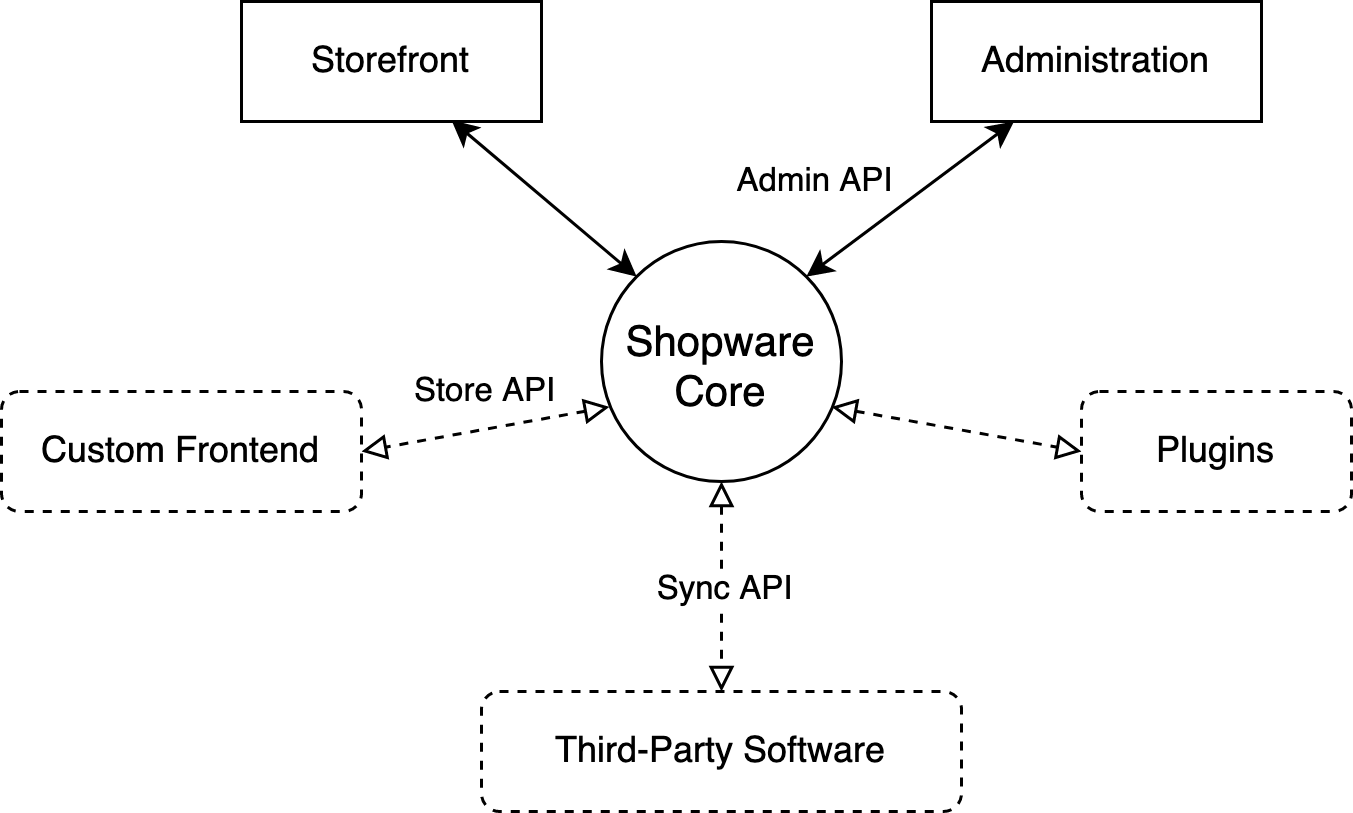
\includegraphics[width=0.7\textwidth]{images/content/shopware-architecture}
    \captioncite[Eigene Darstellung nach]{shopware-architecture-pickware}{Visalisierung der Shopware-Architektur}
    \label{fig:shopware-architecture}
\end{figure}

Eine grobe Zusammenfassung der Architektur kann aus Abbildung\ \ref{fig:shopware-architecture} entnommen werden.
Hierbei werden die Kernkomponenten von Shopware aufgezeigt und optionale Services in gestrichelt dargestellt.
Für die Entwicklung der \acrshort{ci}-Strategie wird der Fokus auf Shopware-Plugins gesetzt.
Durch Plugins können der Shopware-Core, die Administrations-Oberfläche und die Storefront angepasst werden, wobei diese
als abgekapselte Module entwickelt oder als Monolith zusammen mit dem Shopware-Projekt in einem gemeinsamen Repository
verwaltet werden können.
Shopwares Plugin-System baut auf dem Bundle-System von Symfony auf, um standardisierte, modulare Erweiterungen der
Software zu ermöglichen, wobei das Bundle-System Funktionen wie Plugin-Lifecycle-Verwaltung bereitstellt.
Symfony nutzt teils für eigene Core-Features das Bundle-System, um die einzelnen Teilbereiche des Frameworks modular zu
gestalten.\footpartcite{shopware-plugins}
Durch die solide Basis der Symfony-Bundles bieten Shopware-Plugins eine klare Struktur und eine hohe Erweiterbarkeit
und fördern die Wiederverwendbarkeit von entwickelter Software für das Shop-System.

\clearpage
